\begin{figure}[t]
	\centering
	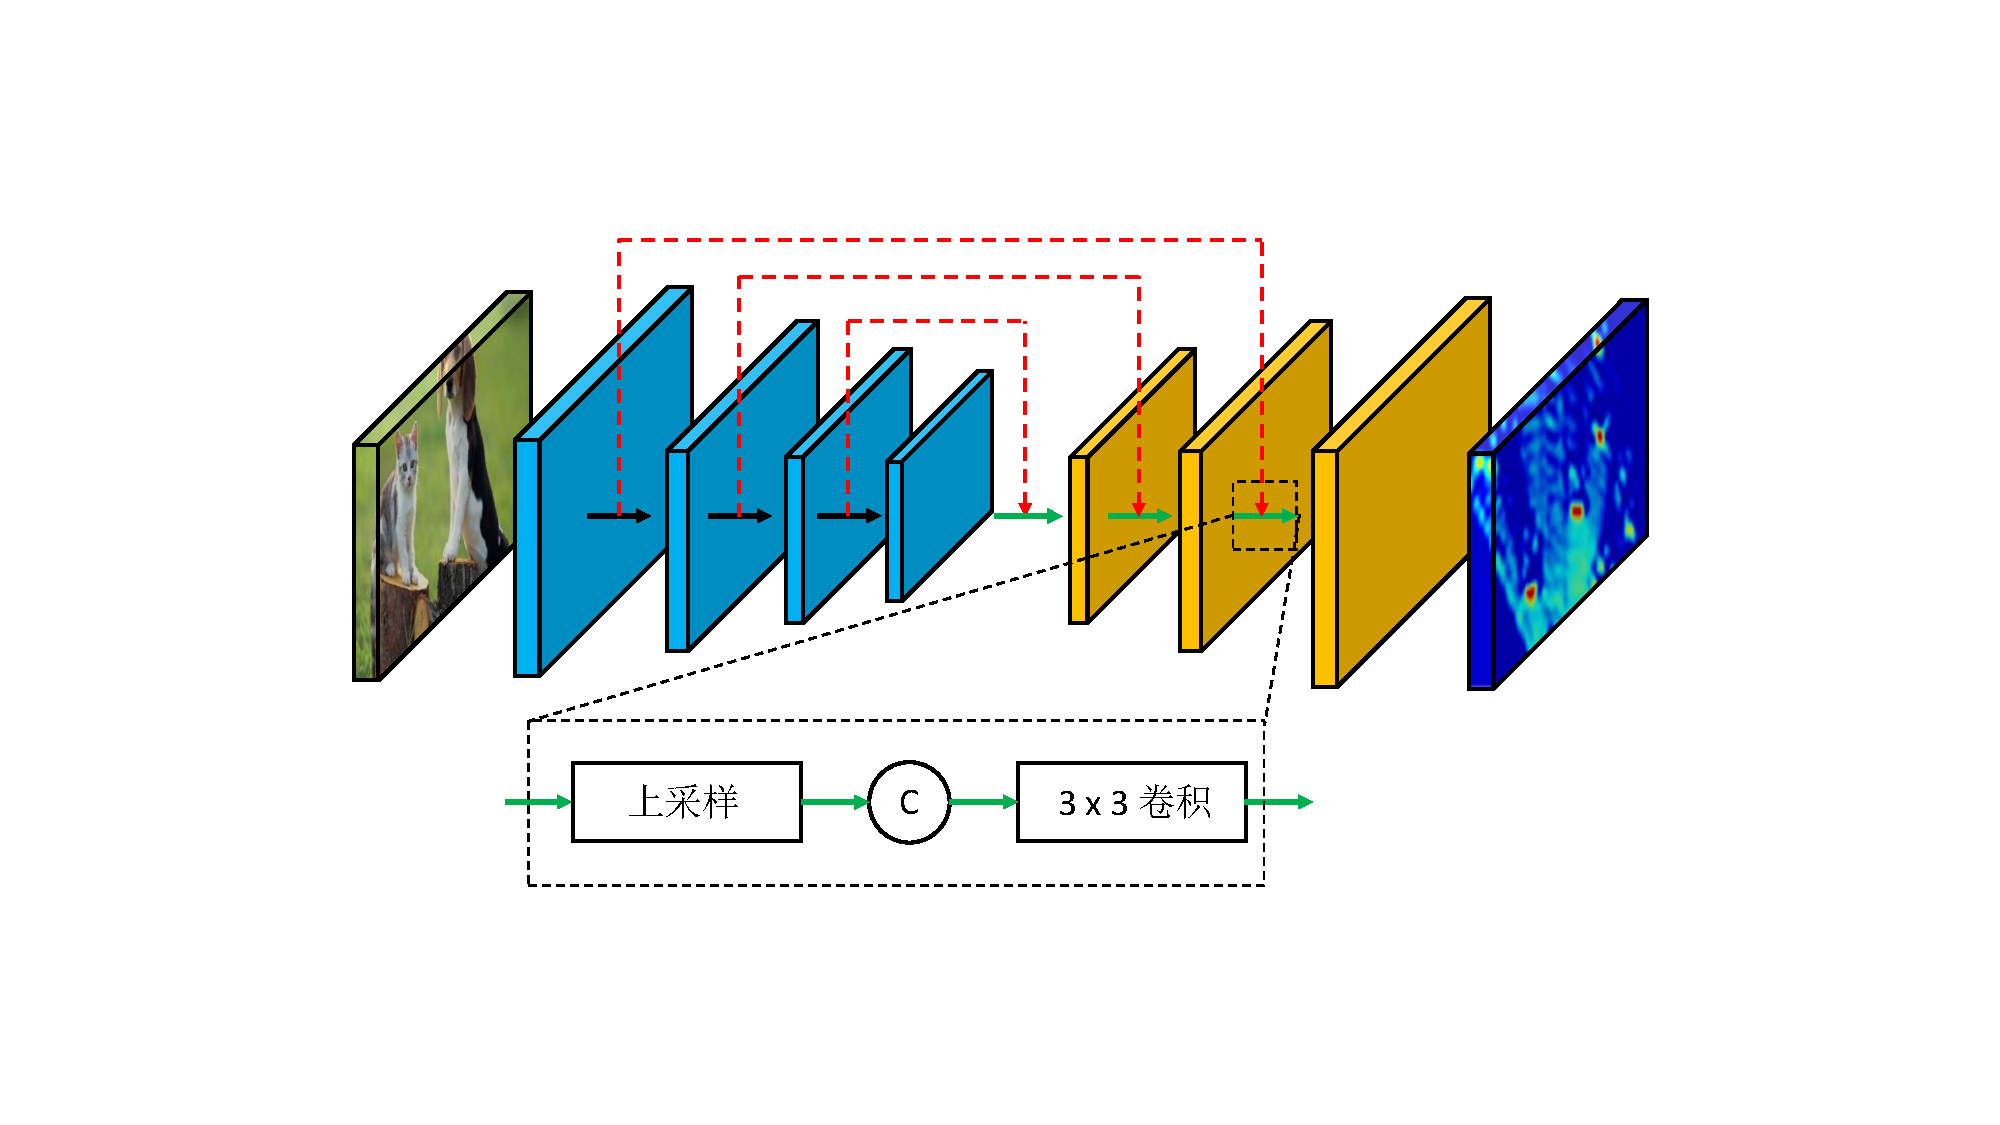
\includegraphics[trim={3cm, 3.5cm, 3cm, 3cm}, clip,width=\textwidth]{imgs/feature-extractor.pdf}
	\caption{特征提取网络结构。左边蓝色部分为编码器,右边橙色部分为解码器,其中“C”表示张量拼接操作(Concat)。}
	\label{fig:feature_extractor}
\end{figure}
